\documentclass[xcolor=dvipsnames]{beamer}

\makeatletter
%HAY QUE ELEGIR EL QUE CORRESPONDA

%\usepackage{mathpazo}%Letra palatino con fuentes para matemáticas
\usepackage[T1]{fontenc}
\usepackage[utf8]{inputenc}
\usepackage{graphicx}
\usepackage{url}
\usepackage{amsmath}
\usepackage{booktabs}
\usepackage{textcomp}%%needed for the euro symbol

\date{}

\usepackage[emulate=units]{siunitx}
\sisetup{per=fraction, fraction=nice, decimalsymbol=comma}
\newunit{\wattpeak}{Wp}
\newunit{\watthour}{Wh}
\newunit{\amperehour}{Ah}

\setbeamercovered{transparent}
\setbeamertemplate{navigation symbols}{}
\usefonttheme{structuresmallcapsserif} 
\usefonttheme{serif} 
\usefonttheme{structurebold}

%\usepackage{epstopdf}


\usepackage[spanish]{babel}
\addto\shorthandsspanish{\spanishdeactivate{~<>}}

\hypersetup{pdfauthor={Oscar Perpi\~n\'an},%
    pdftitle={Energ\'ia Solar Fotovoltaica},%
    filecolor=blue,%
    urlcolor=blue}



%\usepackage{handoutWithNotes} %para hacer papel con notas 
%\pgfpagesuselayout{4 on 1 with notes}[a4paper,border shrink=5mm]



%\usepackage{pgfpages}
%\pgfpagesuselayout{2 on 1}[a4paper,border shrink=5mm]


%\usepackage{mathpazo}%Letra palatino con fuentes para matemáticas
\usepackage[T1]{fontenc}
\usepackage[utf8]{inputenc}
\usepackage{graphicx}
\usepackage{url}
\usepackage{amsmath}
\usepackage{booktabs}

\usepackage[spanish]{babel}
\addto\shorthandsspanish{\spanishdeactivate{~<>}}


\usepackage{hyperref}
% \hypersetup{pdfauthor={Oscar Perpi\~n\'an},%
%     pdftitle={Energ\'ia Solar Fotovoltaica},%
%     filecolor=blue,%
%     urlcolor=blue}

\hypersetup{
    bookmarks=true,         % show bookmarks bar?
%    unicode=true,          % non-Latin characters in Acrobat’s bookmarks
    bookmarksnumbered=false,
    bookmarksopen=false,
    breaklinks=true,
    backref=true,
    pdftoolbar=true,        % show Acrobat’s toolbar?
    pdfmenubar=true,        % show Acrobat’s menu?
    pdffitwindow=false,     % window fit to page when opened
    pdfstartview={FitH},    % fits the width of the page to the window
    pdftitle={Energía Solar Fotovoltaica},    % title
    pdfauthor={Oscar Perpiñán Lamigueiro},     % author
    pdfsubject={Electrotecnia},   % subject of the document
    pdfcreator={AucTeX/Emacs},   % creator of the document
    pdfproducer={LaTeX}, % producer of the document
    pdfnewwindow=true,      % links in new window
    pdfborder={0 0 0},
    colorlinks=true,       % false: boxed links; true: colored links
    linkcolor=,          % color of internal links
    citecolor=BrickRed,        % color of links to bibliography
    filecolor=black,      % color of file links
    urlcolor=Blue           % color of external links 
}

\usepackage[emulate=units]{siunitx}
\sisetup{per=fraction, fraction=nice, decimalsymbol=comma}
\newunit{\wattpeak}{Wp}
\newunit{\watthour}{Wh}
\newunit{\amperehour}{Ah}

\setbeamercovered{transparent}
\setbeamertemplate{navigation symbols}{}
\usefonttheme{serif} 
\usefonttheme{structuresmallcapsserif} 

\useinnertheme[shadow=true]{rounded}
\useoutertheme{shadow}
%\usecolortheme[named=BrickRed]{structure} %sirve para cambiar el color genérico
\usecolortheme{orchid}
\usecolortheme{whale}
\documentclass[xcolor={usenames,svgnames,dvipsnames}]{beamer}
\usepackage[utf8]{inputenc}
\usepackage[T1]{fontenc}
\usepackage{graphicx}
\usepackage{grffile}
\usepackage{longtable}
\usepackage{wrapfig}
\usepackage{rotating}
\usepackage[normalem]{ulem}
\usepackage{amsmath}
\usepackage{textcomp}
\usepackage{amssymb}
\usepackage{capt-of}
\usepackage{hyperref}
\usepackage{color}
\usepackage{listings}
\usepackage{mathpazo}
\usepackage{gensymb}
\usepackage{amsmath}
\usepackage{chemarr}%flechas para reacciones químicas (SFER.tex)
\bibliographystyle{plain}
\AtBeginSubsection[]{\begin{frame}[plain]\tableofcontents[currentsubsection,sectionstyle=show/shaded,subsectionstyle=show/shaded/hide]\end{frame}}
\AtBeginSection[]{\begin{frame}[plain]\tableofcontents[currentsection,hideallsubsections]\end{frame}}
\usepackage[emulate=units]{siunitx}
\sisetup{fraction=nice, decimalsymbol=comma, retain-unity-mantissa = false}
\newunit{\wattpeak}{Wp}
\newunit{\watthour}{Wh}
\newunit{\amperehour}{Ah}
\usepackage{steinmetz}
\hypersetup{colorlinks=true, linkcolor=OliveGreen, urlcolor=Blue}
\renewcommand{\thefootnote}{\fnsymbol{footnote}}
\beamertemplatenavigationsymbolsempty
\setbeamertemplate{footline}[frame number]

\setbeamercolor{alerted text}{fg=Green!50!black} \setbeamerfont{alerted text}{series=\bfseries}
\usefonttheme{serif}
\setbeamercovered{transparent}
\setbeamertemplate{navigation symbols}{}
\usefonttheme{serif} 

\setbeamercolor{palette primary}{bg=OliveGreen,fg=white}
\setbeamercolor{palette secondary}{bg=OliveGreen,fg=white}
\setbeamercolor{palette tertiary}{bg=OliveGreen,fg=white}
\setbeamercolor{palette quaternary}{bg=OliveGreen,fg=white}
\setbeamercolor{structure}{fg=OliveGreen} % itemize, enumerate, etc
\setbeamercolor{section in toc}{fg=OliveGreen} % TOC sections

\usetheme[hideothersubsections]{Goettingen}

\usepackage{tikz}

\titlegraphic{
\includegraphics[width=2.5cm]{../figs/logoEOI.jpg}}
\addtobeamertemplate{frametitle}{}{%
\begin{tikzpicture}[remember picture,overlay]
\node[anchor=south east,yshift=2pt] at (current page.south east) {
\includegraphics[width=1.5cm]{../figs/logoEOI.jpg}};
\end{tikzpicture}}


\makeatother


\begin{document}

\title{\textsc{Energía Solar Fotovoltaica:}\\
\textsc{Célula Solar}}


\author{\textsc{Oscar Perpiñán Lamigueiro}}
\date{}

\begin{frame}[plain]

\titlepage

\end{frame}

%
\AtBeginSection[]{
    \begin{frame}
        \frametitle{Índice}
        \tableofcontents[currentsection] 
    \end{frame} 

                  }

\selectlanguage{spanish}%


\section{Teoría de Semiconductores}


\begin{frame}
  \frametitle{Modelo de bandas de energía}

  Supongamos una red cristalina formada por átomos. Según los
  postulados de la Mecánica Cuántica, los \textbf{electrones de un
    átomo aislado} pueden existir \textbf{únicamente en determinados
    estados de energía}.  A medida que disminuye la distancia
  interatómica comienza a observarse la \textbf{interacción mutua
    entre los átomos} hasta formarse un sistema electrónico único. Las
  \textbf{fuerzas de repulsión y atracción} entre los átomos
  encontrarán su \textbf{equilibrio} cuando los átomos estén separados
  por la \textbf{distancia interatómica típica del cristal} que se
  trate. La separación real entre átomos en el cristal será aquella
  para la cual la \textbf{energía del sólido sea mínima}.


\end{frame}

\begin{frame}
  \frametitle{Modelo de bandas de energía}

  \begin{itemize}
  \item En un \textbf{sólido} el número de átomos es tan elevado que
    los niveles de energía forman \textbf{bandas continuas de
      energía}.
  \item Los \textbf{electrones} asociados a los átomos del sólido
    \textbf{llenan estas bandas en orden ascendente}.
  \item La banda de mayor energía completamente ocupada se denomina
    \textbf{banda de valencia} (\emph{electrones ligados a
      átomos}). La siguiente banda, parcialmente ocupada o vacía, se
    denominada \textbf{banda de conducción} (\emph{electrones
      desligados de átomos}).
  \item Estas bandas pueden estar separadas por otra banda de energías
    que corresponde a \textbf{estados no permitidos} (\textbf{banda
      prohibida}), o \textbf{pueden estar solapadas} permitiendo una
    transición fácil de una a otra.
  \end{itemize}

\end{frame}

\begin{frame}
  \frametitle{Conductores, aislantes y semiconductores}

  Las \textbf{propiedades eléctricas} del sólido dependen de esta
  \textbf{posición relativa entre bandas}.

  \begin{itemize}

  \item En un \textbf{conductor} la $E_{g}$ es muy baja y los
    electrones circulan fácilmente por la banda de conducción.
  \item En un \textbf{aislante} se necesita una cantidad de energía
    muy alta

    para que los electrones puedan acceder a la banda de conducción
    ($E_{g}>\SI{5}{\electronvolt}$) .
  \item En un \textbf{semiconductor} la $E_{g}$ es baja
    ($E_{g}<\SI{5}{\electronvolt}$): los electrones pueden
    {}``saltar'' a la banda de conducción con un aporte energético.

    \begin{itemize}
    \item Para el silicio $E_{g}=\SI{1.12}{\electronvolt}$.
    \end{itemize}

  \end{itemize}

\end{frame}

\begin{frame}
  \frametitle{Rotura de Enlaces}

  \begin{itemize}
  \item Cuando se rompe un enlace, un electrón y un hueco quedan
    libres para moverse por el material (conducción intrínseca).
  \item La \textbf{densidad intrínseca de huecos y electrones es
      idéntica}.  Esta densidad depende de la temperatura y de
    $E_{g}$.
  \item Esta \textbf{circulación es aleatoria}, sin una dirección
    predeterminada.
  \end{itemize}

\end{frame}

\begin{frame}
  \frametitle{Recombinación de un par electrón-hueco}

  \begin{itemize}
  \item Por tanto, se producen \textbf{encuentros electrón-hueco} que
    restablecen un enlace con liberación de energia ($E_{g}$) en forma
    de calor.

    \begin{itemize}
    \item Las impurezas del cristal favorecen la recombinación.
    \item El tiempo de vida de portadores mide cuánto tarda en
      producirse el proceso de recombinación.
    \item La longitud de difusión de portadores mide la distancia
      media que puede recorrer un portador antes de ser recombinado.
    \end{itemize}
  \item Esta \textbf{conducción intrínseca} \textbf{no es
      aprovechable} en un circuito externo.
  \item Para evitar la recombinación \textbf{es preciso dirigir el
      movimiento} de electrones y huecos mediante un campo eléctrico.
  \end{itemize}

\end{frame}

\begin{frame}
  \frametitle{Dopaje de semiconductores}
  \framesubtitle{Tipo n}

  \begin{itemize}
  \item El \textbf{dopaje de semiconductores} consiste en introducir
    de forma controlada impurezas en el cristal.
  \item Los átomos de\textbf{ Fósforo} tienen cinco electrones de
    valencia (uno más que el silicio).
  \item Al impurificar un cristal de Silicio con átomos de Fósforo, el
    quinto electrón no queda bien integrado en la red.
  \item La rotura de este enlace se produce con \textbf{baja
      aportación energética} (menor que $E_{g}$).
  \item El \textbf{quinto electrón queda libre pero la carga positiva
      (ión $P^{+}$) está ligada} a la red cristalina.
  \item La \textbf{densidad de electrones es superior a la de huecos}

    \begin{itemize}
    \item Semiconductor \textbf{tipo n}.
    \item El \textbf{portador mayoritario} es el \textbf{electrón}.
    \end{itemize}
  \end{itemize}

\end{frame}

\begin{frame}
  \frametitle{Dopaje de semiconductores}
  \framesubtitle{Tipo n}

  \begin{center}
    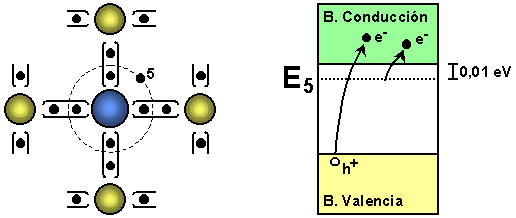
\includegraphics[scale=0.45]{../Figuras/Figuras_Externas/Semiconductor_tipo_n}
    \par\end{center}

\end{frame}

\begin{frame}
  \frametitle{Dopaje de semiconductores}
  \framesubtitle{Tipo p}

  \begin{itemize}
  \item Los átomos de \textbf{Boro} tienen tres electrones de valencia
    (uno menos que el silicio).
  \item Al impurificar un cristal de Silicio con átomos de Boro, hay
    un enlace sin cubrir (hueco).
  \item La rotura de este enlace se produce con \textbf{baja
      aportación energética} (menor que $E_{g}$).
  \item El \textbf{hueco queda libre} pero la \textbf{carga negativa
      (ión $B^{-}$) está ligada} a la red cristalina.
  \item La \textbf{densidad de huecos} es \textbf{superior a la de
      electrones}

    \begin{itemize}
    \item Semiconductor \textbf{tipo p}.
    \item El \textbf{portador mayoritario} es el \textbf{hueco}.
    \end{itemize}
  \end{itemize}

\end{frame}

\begin{frame}
  \frametitle{Dopaje de semiconductores}
  \framesubtitle{Tipo p}

  \begin{center}
    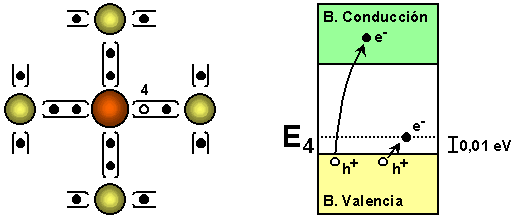
\includegraphics[scale=0.45]{../Figuras/Figuras_Externas/Semiconductor_tipo_p}
    \par\end{center}

\end{frame}

\begin{frame}
  \frametitle{Unión p-n}

  \begin{itemize}
  \item Al\textbf{ unir un semiconductor tipo p con otro tipo n, se
      produce un desequilibrio}
  \item \textbf{Difusión de portadores mayoritarios}

    \begin{itemize}
    \item Hay un movimiento de huecos desde cristal p a cristal n,
      quedando cargado negativamente.
    \item Hay un movimiento de electrones desde cristal n a cristal p,
      quedando cargado positivamente.
    \end{itemize}
  \item Este proceso de difusión también \textbf{desequilibra} las
    densidades de portadores en los cristales.
  \item \textbf{Proceso de arrastre}: Este desequilibrio \textbf{crea
      un campo eléctrico} (sentido del cristal n al cristal p) en
    contra del proceso de difusión.
  \item El \textbf{equilibrio} se alcanza al \textbf{compensarse los
      movimientos de difusión y de arrastre}.
  \end{itemize}

\end{frame}

\begin{frame}[plain]
  \frametitle{Unión p-n}

  \begin{center}
    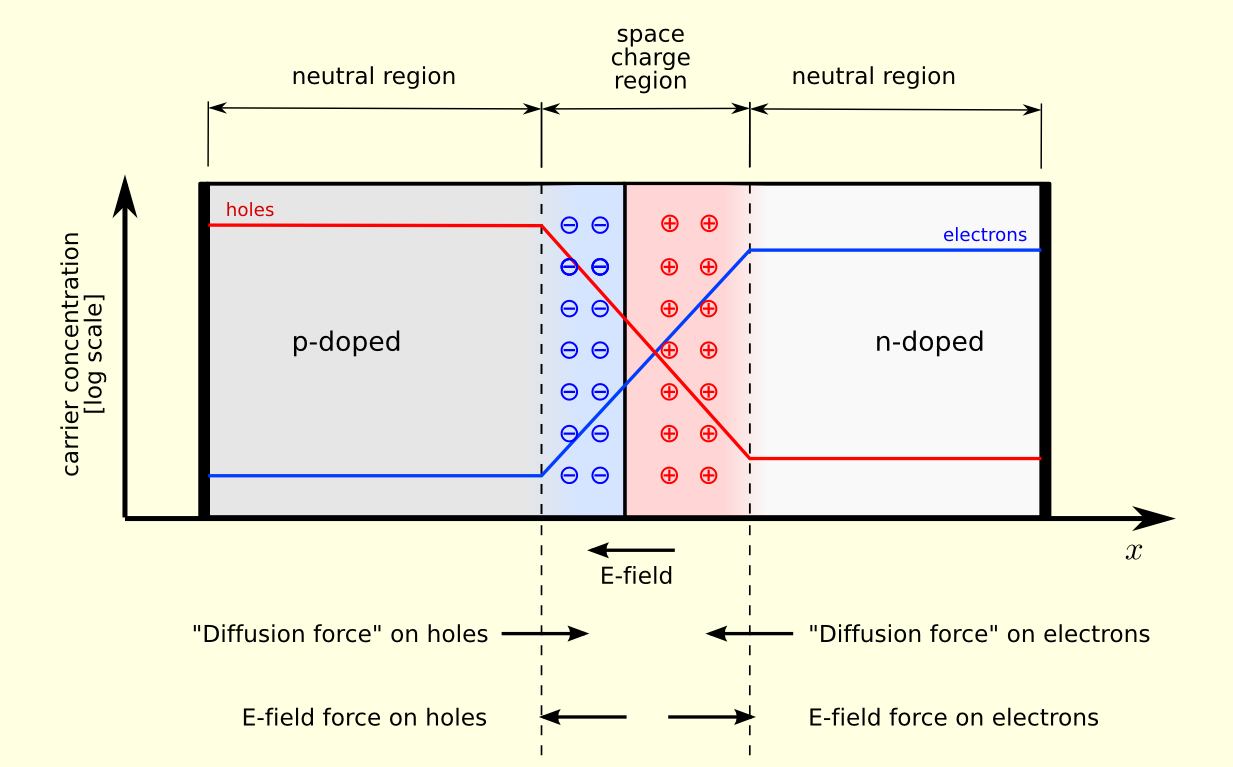
\includegraphics[scale=0.5]{/home/oscar/Docencia/ESF/Figuras/Figuras_Externas/Pn-junction-equilibrium}
    \par\end{center}


\end{frame}
\begin{frame}
  \frametitle{Unión p-n}
  \begin{itemize}
  \item Los \textbf{portadores minoritarios que atraviesan la unión se
      recombinan}:

    \begin{itemize}
    \item Electrones de cristal n con huecos en cristal p.
    \item Huecos de cristal p con electrones en cristal n.
    \end{itemize}
  \item Esta recombinación deja \textbf{iones cargados ligados a la
      red} (incapaces de conducir)
  \item Esta recombinación se produce en \textbf{zonas cercanas a la
      unión} (zona de carga de espacio)

    \begin{itemize}
    \item Despoblada de portadores
    \item \textbf{Los iones fijos generan un campo eléctrico de
        arrastre}.
    \end{itemize}
  \end{itemize}

\end{frame}
\begin{frame}
  \frametitle{Unión p-n}


  \framesubtitle{Polarización en directa}
  \begin{itemize}
  \item \textbf{Para conseguir corriente es necesario romper el
      equilibrio alcanzado y reducir el valor del potencial
      termodinámico}.
  \item \textbf{Diferencia de potencial} con lado p positivo respecto
    al lado n: unión p-n está \textbf{polarizada en directa}.
  \item En estas condiciones \textbf{se reduce la barrera de
      potencial} y, en consecuencia el valor del campo eléctrico de la
    zona de unión.
  \item La \textbf{corriente de arrastre disminuye} y \textbf{no puede
      compensar la corriente de difusión}.
  \item Aparecen dos corrientes en sentidos contrarios pero de
    partículas de diferente signo: \textbf{corriente total
      aprovechable.}
  \item Convenio: la corriente entra por zona p y sale por zona n.
  \end{itemize}

\end{frame}

\begin{frame}
  \frametitle{Unión p-n}


  \framesubtitle{Polarización en inversa}
  \begin{itemize}
  \item Si la diferencia de potencial aplicada consigue que la zona p
    esté a menor tensión que la zona n, la unión queda
    \textbf{polarizada en inversa}.
  \item En estas condiciones \textbf{la barrera de potencial en la
      unión queda reforzada} y el paso de portadores de una a otra
    zona queda aún más debilitado.
  \item La \textbf{corriente }que atraviesa la unión en polarización
    inversa es de \textbf{muy bajo valor}.
  \end{itemize}

\end{frame}

\begin{frame}
  \frametitle{Diodo}
  \begin{block} {}

    El dispositivo electrónico basado en una unión p-n se denomina
    diodo.

    La zona p del diodo es el ánodo y la zona n es el cátodo.

  \end{block}
  \begin{center}
    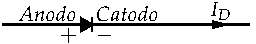
\includegraphics{/home/oscar/Docencia/ESF/Figuras/Diodo}
    \par\end{center}


\end{frame}

\begin{frame}
  \frametitle{Ecuación del Diodo}

\[
I_{D}=I_{0}\cdot[\exp(\frac{V}{m\cdot V_{T}})-1]\] donde $I_{0}$ es la
corriente de saturación en oscuridad del diodo, $V$ la tensión
aplicada al diodo y $m$ el factor de idealidad del diodo.

Para una temperatura ambiente de $\SI{300}{\kelvin}$, \[
V_{T}=\frac{\mathrm{k}T}{\mathrm{e}}=\SI{25.85}{\milli\volt}\] donde
$\mathrm{k}$ es la constante de Boltzmann, $T$ la temperatura del
diodo (en grados Kelvin), y $\mathrm{e}$ es la carga del electrón.


\end{frame}

\begin{frame}
  \frametitle{Ecuación del Diodo}

  \begin{center}
    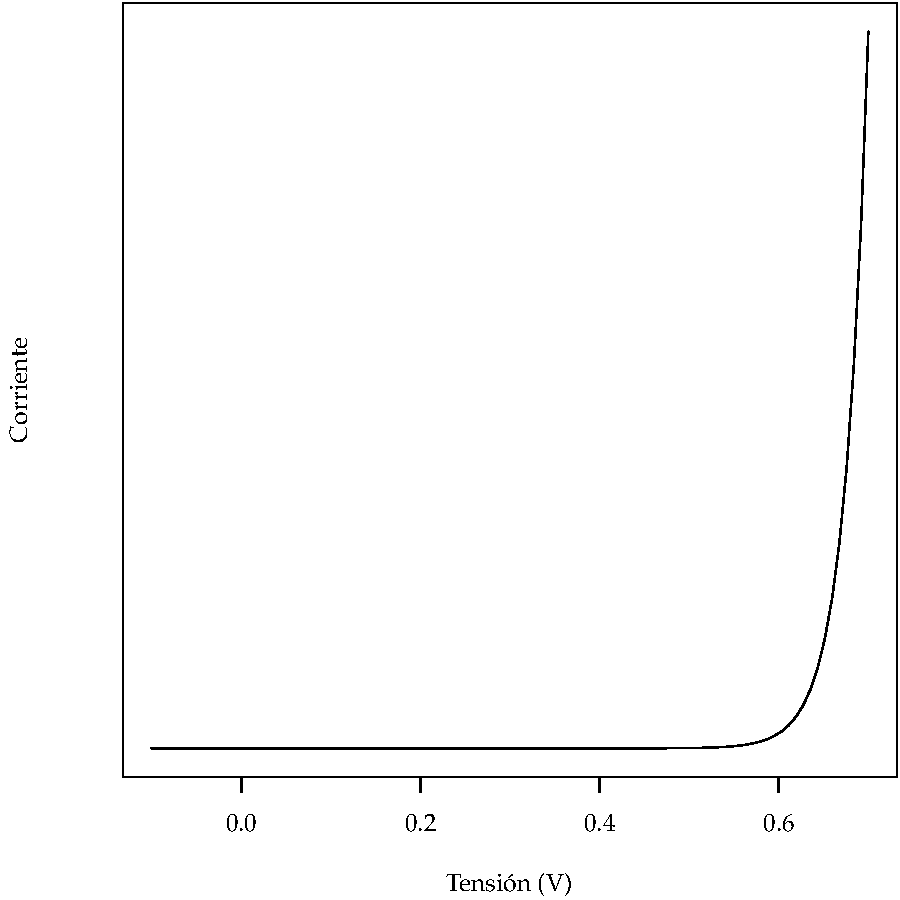
\includegraphics[scale=0.45]{/home/oscar/Docencia/ESF/Figuras/EcuacionDiodo}
    \par\end{center}


\end{frame}

\section{Unión P-N iluminada}


\begin{frame}
  \frametitle{Efecto fotoeléctrico}
  \begin{itemize}
  \item Efecto fotoeléctrico: \textbf{los electrones se desplazan a la
      banda de conducción por el aporte energético de fotones}
    ($E_{f}=\frac{h\cdot c}{\lambda}$).
  \item Al \textbf{iluminar una unión p-n}, el \textbf{campo
      eléctrico} de la unión conduce los portadores y
    \textbf{dificulta la recombinación}.
  \item La \textbf{fotocorriente} es ahora \textbf{aprovechable} por
    un circuito externo (\emph{corriente de iluminación, corriente de
      generación})
  \item La presencia de \textbf{tensión en los terminales} de la unión
    (por ejemplo, caída de tensión en una resistencia alimentada por
    la fotocorriente)\textbf{ favorece la recombinación}
    (\emph{corriente de oscuridad o corriente de diodo}).\end{itemize}
  \begin{block} {}

\[
I=I_{L}-I_{0}\cdot[\exp(\frac{V}{m\cdot V_{T}})-1]\]


\end{block}

\end{frame}

\begin{frame}
  \frametitle{Unión p-n iluminada}

  \begin{center}
    \includegraphics[scale=0.7]{../Figuras/Figuras_Externas/CelulaSolar}
    \par\end{center}


\end{frame}

\begin{frame}
  \frametitle{Absorción de luz y generación de portadores}
  \begin{itemize}
  \item Si el \textbf{fotón es poco energético} ($E_{f}<E_{g}$)
    \textbf{no interactúa con el semiconductor} (como si fuese
    transparente)

    \begin{itemize}
    \item Fotones en el espectro visible ($400\, nm<\lambda<700\, nm$)
      y ultravioleta ($\lambda<400\, nm$) rompen enlaces.
    \item Si $\lambda>1100\, nm$ (infrarrojo) el fotón no interactúa.
    \end{itemize}
  \item Los\textbf{ fotones más energéticos }(baja longitud de onda)
    son \textbf{absorbidos en la superficie}.
  \item Los \textbf{fotones menos energéticos} (alta longitud de onda)
    penetran en el interior hasta \textbf{romper un enlace}.
  \end{itemize}

\end{frame}

\begin{frame}
  \frametitle{Absorción de luz y generación de portadores}
  \begin{itemize}
  \item Los fotones con $E_{f}<E_{g}$ atraviesan el cristal sin ser
    absorbidos: \textbf{pérdidas de no-absorción}
  \item Fotones con $E_{f}>E_{g}$:

    \begin{itemize}
    \item Debido a anchura del semiconductor y coeficiente de
      absorción del material parte no son absorbidos: \textbf{pérdidas
        de transmisión}
    \item Debido a diferencia de índices de refracción:
      \textbf{pérdidas de reflexión}
    \item Parte de los portadores generadores se recombinan dentro del
      dispositivo: \textbf{pérdidas por recombinación}
    \end{itemize}
  \end{itemize}
  \[
  I_{L}<e\cdot A\cdot\intop_{E_{G}}^{\infty}S(E)\mathrm{d}E\]



\end{frame}

\section{Característica I-V}


\begin{frame}[plain]
  \frametitle{Característica I-V de iluminación}

\[
I=I_{L}-I_{D}\]


\[
I_{D}=I_{0}\cdot\left[\exp\left(\frac{e\cdot V}{m\cdot k\cdot
      T_{c}}\right)-1\right]\]


\begin{center}
  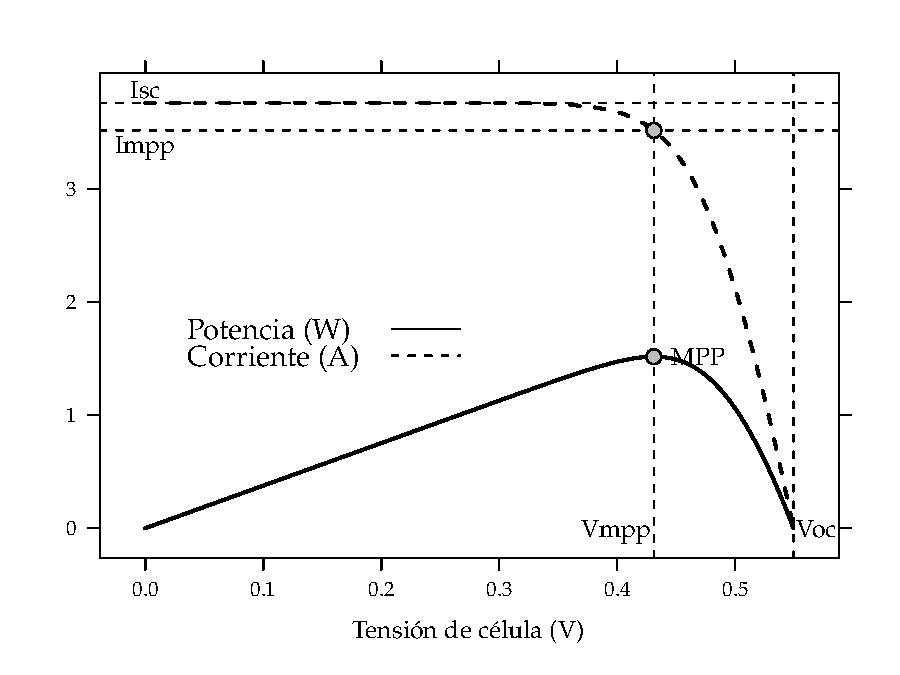
\includegraphics[scale=0.5]{/home/oscar/Docencia/ESF/Figuras/CurvaIV_Ta20_G800}
  \par\end{center}


\end{frame}

\begin{frame}
  \frametitle{Isc y Voc}
  \begin{block} {Corriente de Cortocircuito}

\[
I_{sc}=I(V=0)\Rightarrow I_{D}=0\Rightarrow I=I_{L}\]


\end{block} {}
\begin{block} {Tensión de Circuito Abierto}

\[
V_{oc}=V(I=0)\Rightarrow I_{L}=I_{D}\Rightarrow
V_{oc}=m\cdot\frac{k\cdot
  T_{c}}{e}\cdot\ln\left(\frac{I_{L}}{I_{0}}+1\right)\]


\end{block} {}
\begin{block} {Ecuación general}

\[
I=I_{sc}\cdot\left[1-\exp\left(\frac{e\cdot(V_{oc}-V)}{m\cdot k\cdot
      T_{c}}\right)\right]\]


\end{block} {}


\end{frame}

\begin{frame}
  \frametitle{Punto de máxima potencia}

\[
\frac{dP}{dV}=0\]


\[
\frac{d(I\cdot
  V)}{dV}=V\cdot\frac{dI(V)}{dV}+I\cdot\frac{dV}{dV}\Rightarrow
dP=V\cdot dI+I\cdot dV\]



\end{frame}

\begin{frame}[plain]
  \frametitle{Punto de máxima potencia}

  \begin{center}
    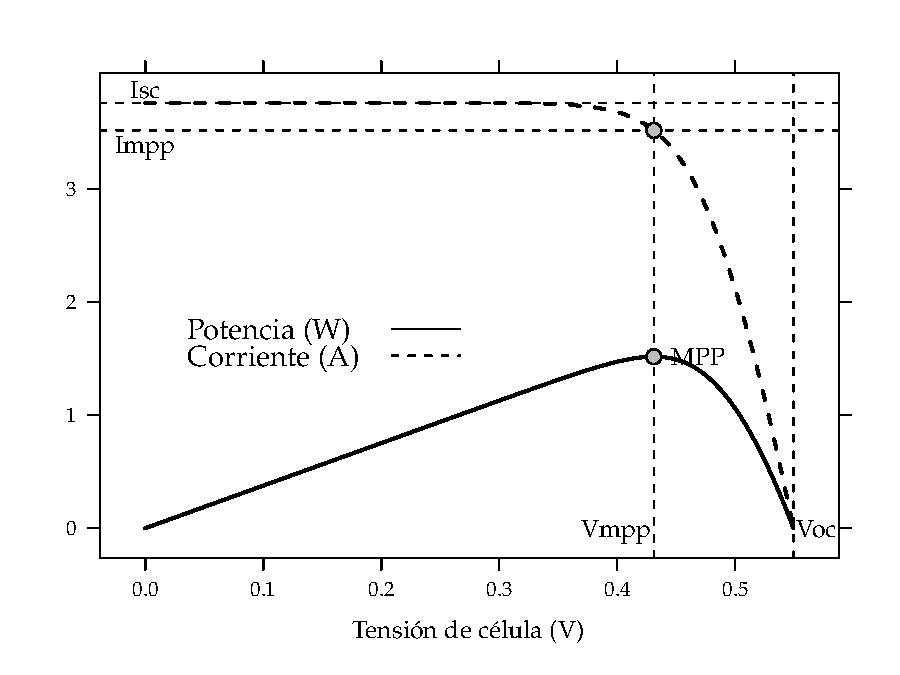
\includegraphics[scale=0.4]{/home/oscar/Docencia/ESF/Figuras/CurvaIV_Ta20_G800}
    \par\end{center}
  \begin{block} {}

\begin{center}
  $V=V_{mpp}:\,\frac{dI}{dV}=-\frac{I}{V}$
  \par\end{center}

\begin{center}
  $0<V<V_{mpp}$:
  ~$\frac{dP}{dV}>0\Rightarrow\frac{dI}{dV}>-\frac{I}{V}$
  \par\end{center}

\begin{center}
  $V_{mpp}<V<V_{oc}$:~
  $\frac{dP}{dV}<0\Rightarrow\frac{dI}{dV}<-\frac{I}{V}$
  \par\end{center}

\end{block}

\end{frame}

\begin{frame}
  \frametitle{Factor de forma y Eficiencia}

\[
FF=\frac{I_{mpp}\cdot V_{mpp}}{I_{sc}\cdot V_{oc}}\]


\[
P_{mpp}=FF\cdot I_{sc}\cdot V_{oc}\]


\[
\eta=\frac{I_{mpp}\cdot V_{mpp}}{P_{L}}\]



\end{frame}

\begin{frame}[plain]
  \frametitle{Eficiencia de células}

  \begin{center}
    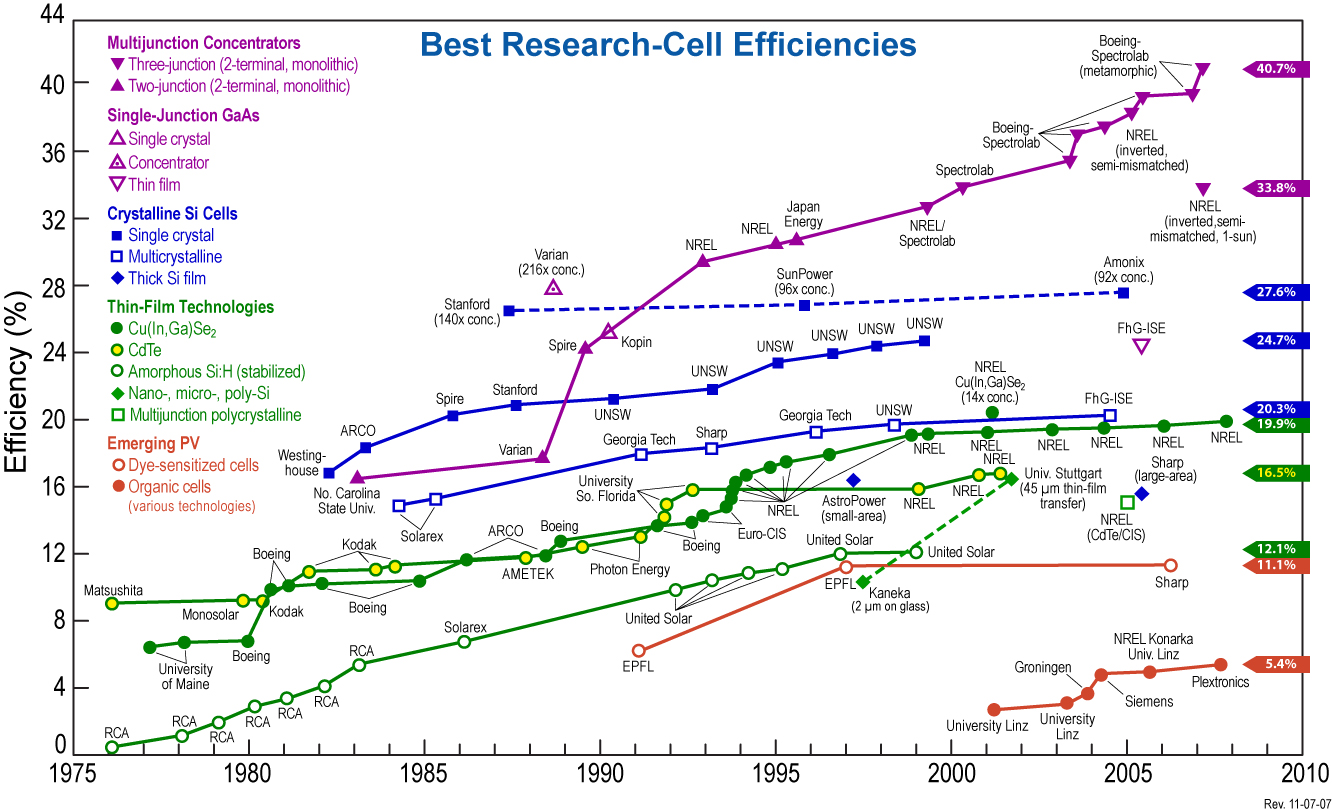
\includegraphics[scale=0.25]{/home/oscar/Docencia/ESF/Figuras/Figuras_Externas/PVeff(rev110707)d}
    \par\end{center}


\end{frame}

\begin{frame}
  \frametitle{Circuito equivalente de la célula}

  \begin{center}
    \includegraphics[scale=0.75]{/home/oscar/Docencia/ESF/Figuras/CelulaSolar}
    \par\end{center}

\[
I=I_{L}-I_{0}\cdot[\exp(\frac{V+I\cdot R_{s}}{m\cdot
  V_{T}})-1]-\frac{V+I\cdot R_{s}}{R_{p}}\]

\begin{block} {Ecuación simplificada}

\[
I=I_{sc}[1-\exp(\frac{V-V_{oc}+I\cdot R_{s}}{m\cdot V_{t}})]\]


\end{block}

\end{frame}

\begin{frame}
  \frametitle{Resistencia Serie}
  \begin{block} {}
    \begin{itemize}
    \item Resistencia de contactos metálicos con el semiconductor
    \item Resistencia de capas semiconductoras
    \item Resistencia de malla de metalización
    \end{itemize}
  \end{block}
  \begin{columns}[t]


    \column{6cm}

    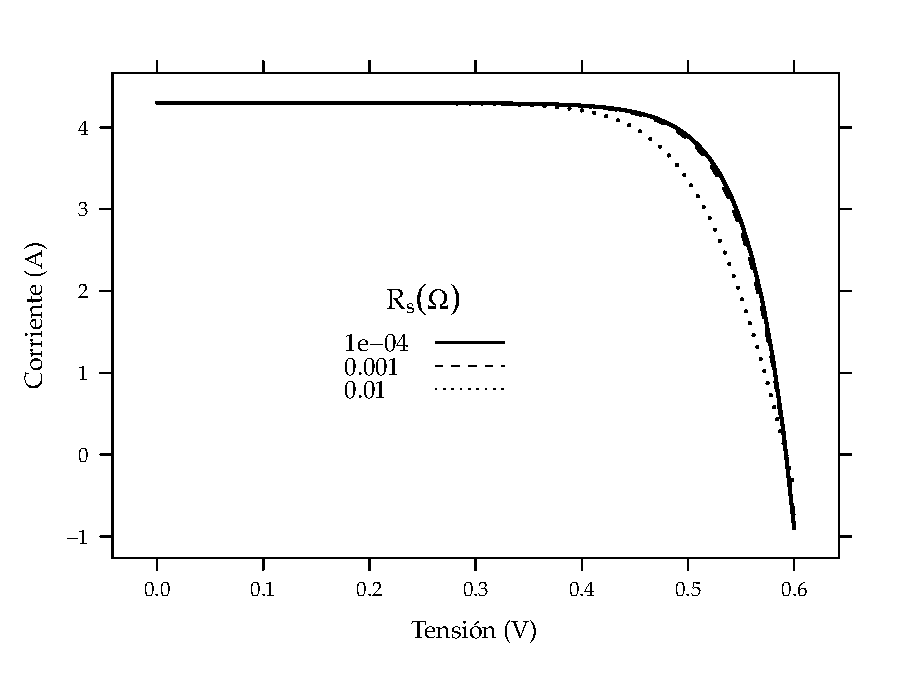
\includegraphics[scale=0.4]{/home/oscar/Docencia/ESF/Figuras/InfluenciaRs_IV}


    \column{6cm}

    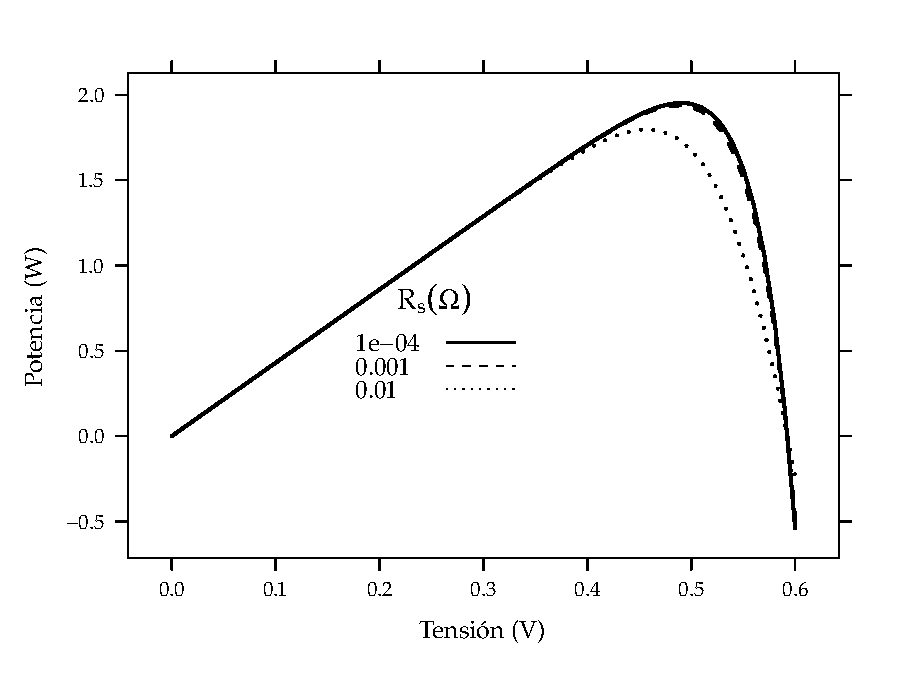
\includegraphics[scale=0.4]{/home/oscar/Docencia/ESF/Figuras/InfluenciaRs_Potencia}

  \end{columns}

\end{frame}

\begin{frame}
  \frametitle{Resistencia paralelo}
  \begin{block} {}
    \begin{itemize}
    \item Fugas de corriente en bordes de célula
    \item Cortocircuitos metálicos
    \item Caminos de difusión en fronteras de grano
    \end{itemize}
  \end{block}
  \begin{columns}[c]


    \column{6cm}

    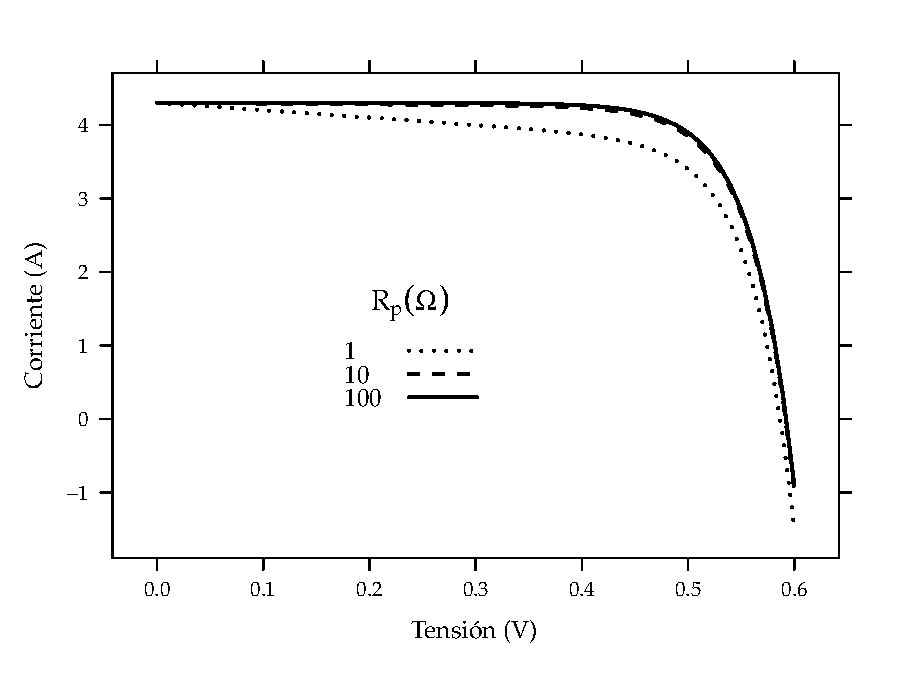
\includegraphics[scale=0.4]{/home/oscar/Docencia/ESF/Figuras/InfluenciaRsh_IV}


    \column{6cm}

    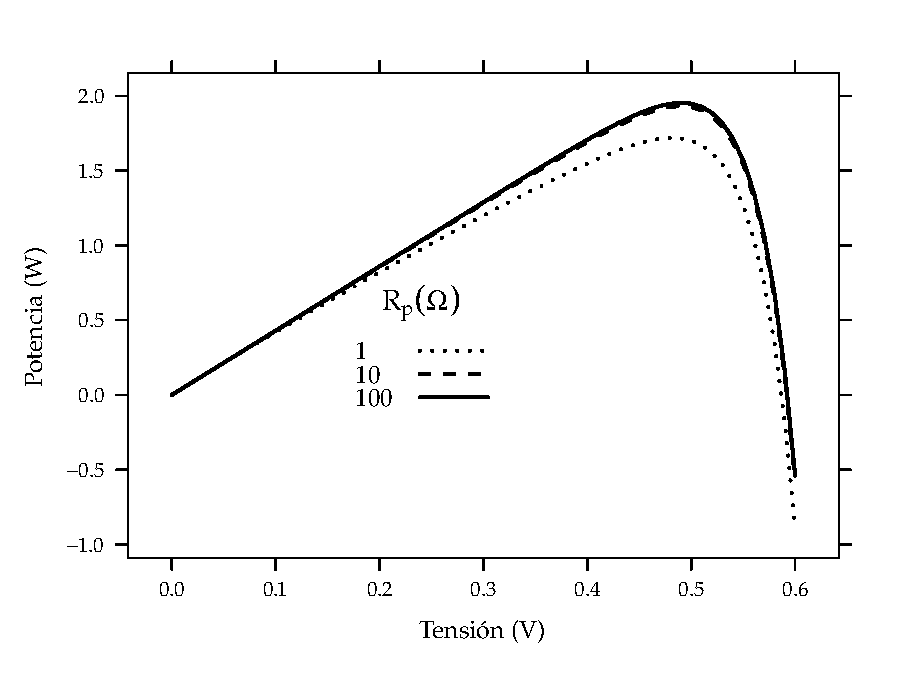
\includegraphics[scale=0.4]{/home/oscar/Docencia/ESF/Figuras/InfluenciaRsh_Potencia}

  \end{columns}

\end{frame}

\begin{frame}
  \frametitle{Influencia de factores externos}
  \begin{itemize}
  \item \textbf{Temperatura}

    \begin{itemize}
    \item Se estrecha el salto entre banda de valencia y conducción:
      aumenta \emph{ligeramente} la fotocorriente
    \item Disminuye la tensión de circuito
      abierto:$dV_{oc}/dT_{c}=\SI{-2.3}{\milli\volt\per\celsius}$
    \item Disminuye el factor de forma y la eficiencia:
      $d\eta/dT_{c}=\SI{-0.4}{\percent\per\celsius}$
    \end{itemize}
  \item \textbf{Iluminación}

    \begin{itemize}
    \item Fotocorriente proporcional a intensidad de radiación
    \item Relación logarítmica con tensión de circuito abierto:
      $V_{oc}=V_{oc1}+\frac{mkT}{e}\cdot\ln(X)$
    \item El factor de forma aumenta ligeramente
    \item La eficiencia crece de forma logarítmica hasta determinado
      nivel.
    \end{itemize}
  \end{itemize}

\end{frame}

\begin{frame}[plain]
  \frametitle{Influencia de la Radiación}

  \begin{center}
    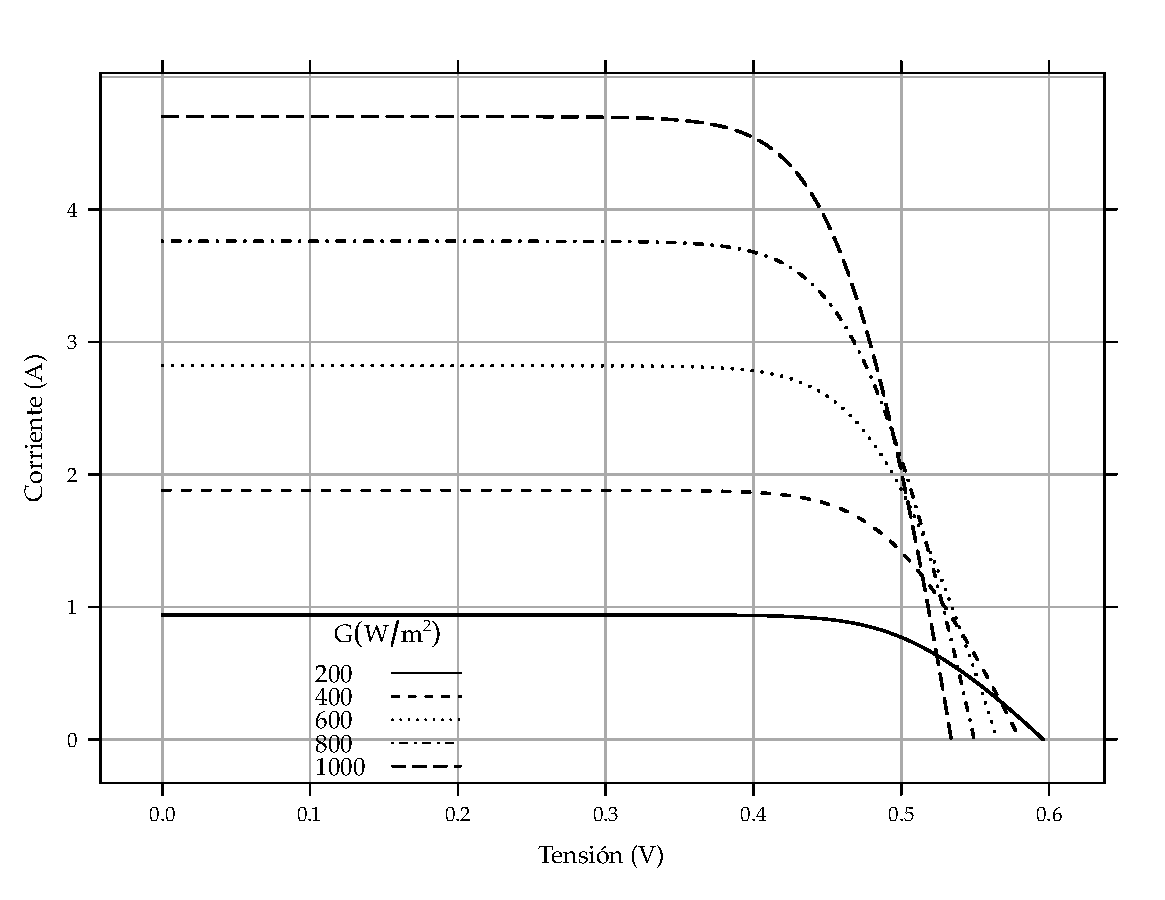
\includegraphics[scale=0.6]{/home/oscar/Docencia/ESF/Figuras/CurvaIV_Ta20}
    \par\end{center}


\end{frame}

\begin{frame}[plain]
  \frametitle{Influencia de Temperatura}

  \begin{center}
    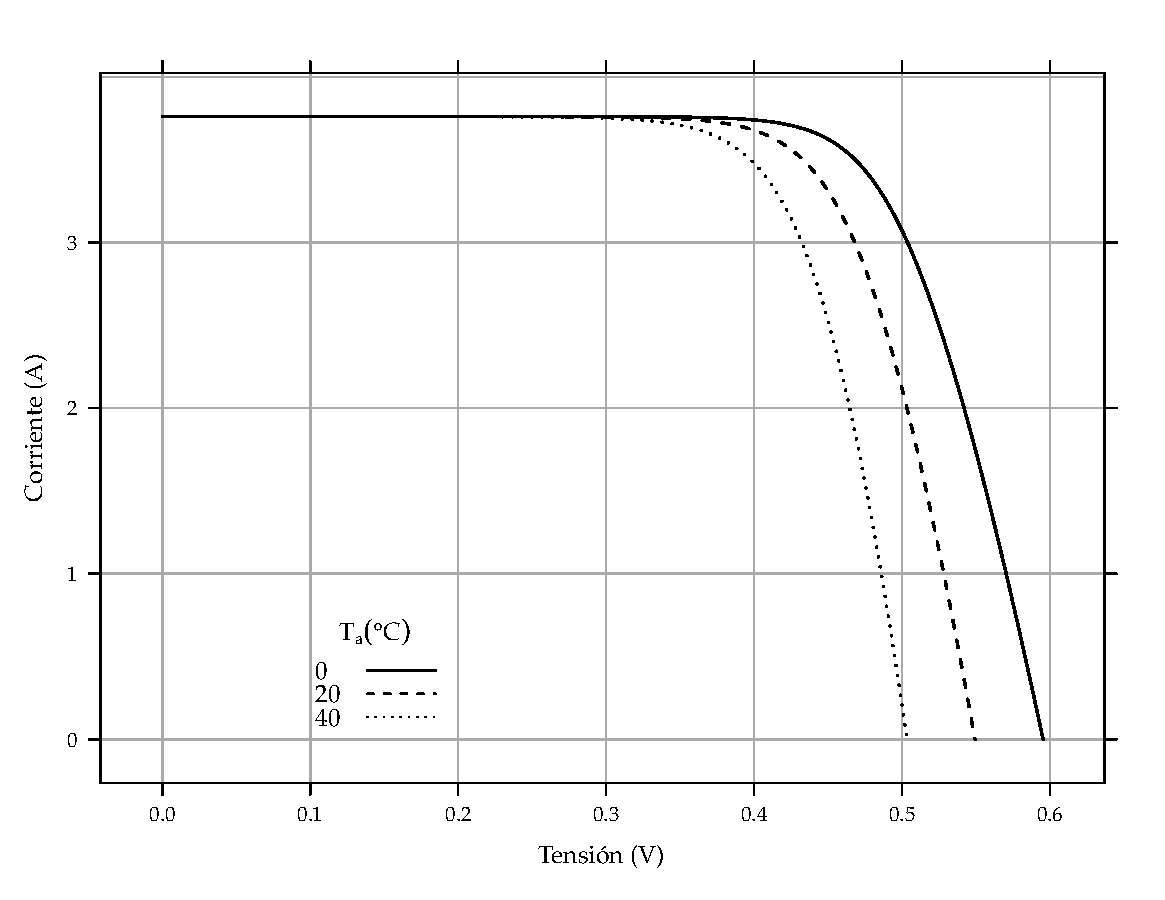
\includegraphics[scale=0.6]{/home/oscar/Docencia/ESF/Figuras/CurvaIV_G800}
    \par\end{center}


\end{frame}

\begin{frame}
  \frametitle{Condiciones Estándar de Medida}
  \begin{itemize}
  \item Irradiancia: $G^{*}=\SI{1000}{\watt\per\meter\squared}$ con
    incidencia normal.
  \item Temperatura de célula: $T_{c}^{*}=\SI{25}{\celsius}$.
  \item Masa de aire: $AM=1.5$\end{itemize}
  \begin{block} {}

\[
P_{mpp}^{*}=I_{mpp}^{*}\cdot V_{mpp}^{*}\]


\[
\eta^{*}=\frac{I_{mpp}^{*}\cdot V_{mpp}^{*}}{A\cdot G^{*}}\]


\end{block}

\end{frame}

\begin{frame}[plain]
  \frametitle{Cálculo de punto de máxima potencia}


  \framesubtitle{Método de J.M. Ruiz}
  \begin{block} {Normalización}

\begin{eqnarray*}
  v & = & \frac{V}{V_{oc}}\\
  i & = & \frac{I}{I_{sc}}\end{eqnarray*}


\end{block} {}
\begin{block} {MPP}

\begin{eqnarray*}
  v_{mpp} & = & \frac{V_{mpp}}{V_{oc}}\\
  i_{mpp} & = & \frac{I_{mpp}}{I_{sc}}\\
  p_{mpp} & = & FF\end{eqnarray*}


\end{block}

\end{frame}

\begin{frame}
  \frametitle{Cálculo de punto de máxima potencia}


  \framesubtitle{Método de J.M. Ruiz}
  \begin{block} {Resistencia Serie y FF}

\begin{eqnarray*}
  r_{s} & = & \frac{R_{s}}{(V_{oc}/I_{sc})}\\
  ff & = & v_{mpp}\cdot i_{mpp}=FF\end{eqnarray*}


\end{block} {}
\begin{block} {Tensión térmica}

\begin{eqnarray*}
  k_{oc} & = & \frac{V_{oc}}{V_{t}}\end{eqnarray*}


\end{block}

\end{frame}

\begin{frame}
  \frametitle{Cálculo de punto de máxima potencia}


  \framesubtitle{Método de J.M. Ruiz}
  \begin{block} {Aproximación para MPP}

\begin{eqnarray*}
  i_{mpp} & = & 1-\frac{D_{M}}{k_{oc}}\\
  v_{mpp} & = & 1-\frac{\ln(k_{oc}/D_{M})}{k_{oc}}-r_{s}\cdot i_{mpp}\end{eqnarray*}
 

\begin{eqnarray*}
  D_{M} & = & D_{M0}+2\cdot r_{s}\cdot D_{M0}^{2}\\
  D_{M0} & = & \frac{k_{oc}-1}{k_{oc}-\ln k_{oc}}\end{eqnarray*}


\end{block}

\end{frame}

\begin{frame}
  \frametitle{Cálculo de punto de máxima potencia}


  \framesubtitle{Método de J.M. Ruiz}
  \begin{block} {Itinerario}
    \begin{itemize}
    \item Obtener los valores de $I_{sc}$ y $V_{oc}$ en las
      condiciones de temperatura y radiación deseadas
    \item Obtener resistencia serie (supondremos $R_{s}=R_{s}^{*}$) \[
      R_{s}^{*}=\frac{V_{oc}^{*}-V_{mpp}^{*}+m\cdot
        V_{t}\cdot\ln(1-\frac{I_{mpp}^{*}}{I_{sc}^{*}})}{I_{mpp}^{*}}\]
      donde se debe emplear el valor de $V_{t}$ para
      $T_{c}=\SI{25}{\celsius}$.
    \item Calcular $r_{s}$ y $k_{oc}$, y con ellos $D_{M0}$ y $D_{M}$.
    \item Calcular $i_{mpp}$ y a continuación $v_{mpp}$.
    \item Deshacer la normalización para obtener $I_{mpp}$ y
      $V_{mpp}$.
    \end{itemize}
  \end{block}

\end{frame}

\begin{frame}
  \frametitle{Cálculo de punto de máxima potencia}


  \framesubtitle{Factor de Forma Constante}
  \begin{block} {}

\[
FF=FF^{*}\]


\end{block} {}
\begin{block} {}

\begin{eqnarray*}
  \frac{I_{mpp}}{I_{sc}} & = & \frac{I_{mpp}^{*}}{I_{sc}^{*}}\\
  \frac{V_{mpp}}{V_{oc}} & = & \frac{V_{mpp}^{*}}{V_{oc}^{*}}\end{eqnarray*}


\end{block}

\end{frame}

\begin{frame}
  \frametitle{Cálculo de parámetros}

  De una célula de $\SI{100}{\centi\meter\squared}$ y $I_{sc}^{*}=3\,
  A$, $I_{mpp}^{*}=2.7\, A$ , $V_{oc}^{*}=0.6\, V$,
  $V_{mpp}^{*}=0.48\, V$, calcular suponiendo factor de forma constante:
  \begin{itemize}
  \item $P_{mpp}^{*}$, $FF^{*}$, $\eta^{*}$
  \item $I_{mpp}$, $V_{mpp}$ cuando $T_{c}=60\celsius$ y
    $G=800\, W/m^{2}$.
  \end{itemize}

\end{frame}

\section{Fabricación}

\begin{frame}
  \frametitle{Fabricación de células de silicio}
  \begin{itemize}
  \item El silicio puede extraerse de la cuarzita obteniendo Silicio
    de grado metalúrgico (98\% pureza).
  \item Para la industria de la electrónica se necesita silicio de
    grado electronico (nivel de impureza por debajo de $10^{-10}$, 9
    nueves).
  \item Para las células solares puede utilizarse silicio de grado
    solar (nivel de impureza algo mayor).
  \item Al mezclar silicio con acido clorhídrico se produce
    triclorosilano, que es destilado para eliminar impurezas.
  \item Al unir silano de cloro con hidrógeno se obtiene de vuelta
    silicio, válido para células policristalinas (varios cristales en
    cada célula)
  \end{itemize}

\end{frame}

\begin{frame}
  \frametitle{Fabricación de células de silicio}
  \begin{itemize}
  \item Para obtener mayor pureza se emplea el silicio monocristalino
    (un sólo cristal) obtenido mediante el proceso de Czochralski o
    similar (se utiliza una semilla de cristal para crecer silicio a
    muy alta temperatura).
  \item El lingote resultante debe ser cortado en obleas de
    $200-500\,\mu m$.
  \item Las obleas son sometidas a limpieza para eliminar impurezas
    por el cortado.
  \item A continuación, son dopadas con Fósforo y Boro para crear la
    unión p-n.
  \item Se limpian los bordes para evitar la formación de
    cortocircuitos entre las zonas p y n.
  \end{itemize}

\end{frame}

\begin{frame}
  \frametitle{Fabricación de células de silicio}
  \begin{itemize}
  \item Se añaden los contactos posterior (alto recubrimiento) y
    anterior (optimización para obtener baja $R_{s}$ y poco sombreado)
    empleando aleaciones de plata y aluminio.
  \item Para reducir las pérdidas por reflexión se añade una capa
    antireflectante con (p.ej) óxido de Titanio (color azulado).
  \item Si es posible, se textura la superficie (creación de mini
    pirámides).
  \end{itemize}

\end{frame}


\end{document}
